% $Id: board2.tex 10137 2022-06-04 20:51:54Z mskala $

%
% MSK 013 Board 2 build instructions
% Copyright (C) 2020  Matthew Skala
%
% This program is free software: you can redistribute it and/or modify
% it under the terms of the GNU General Public License as published by
% the Free Software Foundation, version 3.
%
% This program is distributed in the hope that it will be useful,
% but WITHOUT ANY WARRANTY; without even the implied warranty of
% MERCHANTABILITY or FITNESS FOR A PARTICULAR PURPOSE.  See the
% GNU General Public License for more details.
%
% You should have received a copy of the GNU General Public License
% along with this program.  If not, see <http://www.gnu.org/licenses/>.
%
% Matthew Skala
% https://northcoastsynthesis.com/
% mskala@northcoastsynthesis.com
%

\chapter{Building Board 2}

The recommended order for building this module is to assemble Board 2, the
one further from the front panel, first.  That will make it easier to get
all the physical positioning right for the components that bridge between
the boards or pass through the panel.

Note that although I'm describing a separate step for each component value,
and that's how I built my prototype so as to have plenty of photo
opportunities, if you are reasonably confident about your skills you may
find it easier to populate all or most of the board (i.e.\ put the
components in place) and then solder them in a single step.  Except where
noted, the order in which you add components does not matter much.

\section{Preliminaries}

Count out the right number of everything according to the bill of materials. 
There is an abbreviated BOM for Board~2, excluding a few items that will be
added when combining this board with Board~1, in Table~\ref{tab:b2bom}.

\nopagebreak
\noindent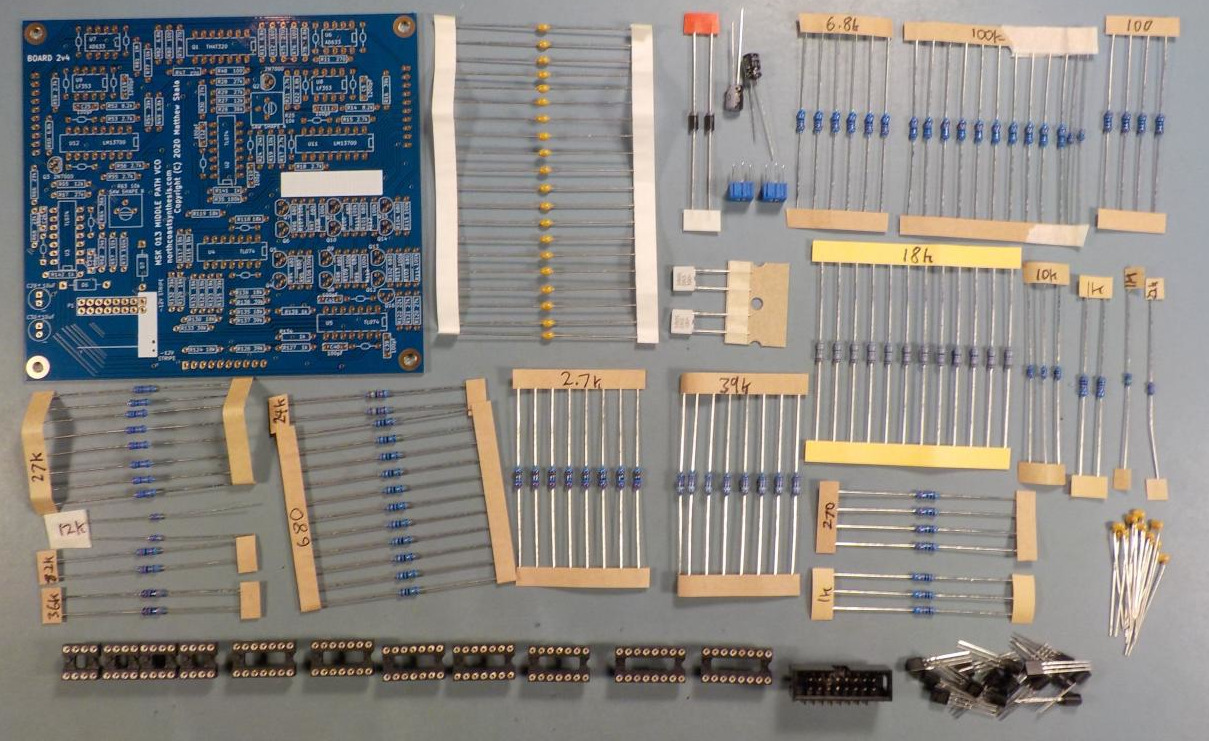
\includegraphics[width=\linewidth]{board2-parts.jpg}

\begin{table*}
{\centering
\fbox{This table is not a substitute for the text instructions.}
\vspace{\baselineskip}

\begin{tabular}{rp{1.4in}cp{2.9in}}
  \textbf{Qty} & \textbf{Ref} & \textbf{Value/Part No.} & \\ \hline
\input{bomdata-2.tex}
\end{tabular}\par}
\caption{Bill of Materials for assembling Board~2~-- excluding a few that
are better added later, during the Board~1 build.  Also needed is the PCB
itself.}\label{tab:b2bom}
\end{table*}

The components for this board include 2N7000 MOSFETs, which are
static-sensitive.  You should take anti-static precautions with these.  They
should be supplied in anti-static packaging.  Leave them in that packaging
until you need to use them, and work on an anti-static surface, with a
grounding wrist strap, or both, while handling these components.  After the
MOSFETs are installed, assuming the resistors were installed first as
recommended, the resistors will provide some protection for these MOSFETs,
reducing the necessary precaution level.  North Coast kits
include spare MOSFETs just in case.

\section{Decoupling capacitors}

The 20 axial ceramic 0.1$\mu$F decoupling capacitors, C1--C4, C6--C9, C13,
C14, C17, C18, C20--C23, and C35--C38, are shown on the board by a special
symbol without their reference designators.

\nopagebreak
\noindent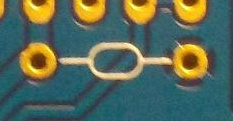
\includegraphics[width=\linewidth]{decoup-symbol.jpg}

Install these capacitors where the symbol appears.  They are not
polarized and may be installed in either orientation.  These capacitors act
as filters for the power supplies to the integrated circuits.  An MSK~013
kit should include 25 of these capacitors; save the remaining five for use
on Board~1.

\nopagebreak
\noindent\includegraphics[width=\linewidth]{{cap-0.1u2}.jpg}

\pagebreak

\section{Fixed resistors}

Resistors are never polarized.  I like to install mine in a consistent
direction for cosmetic reasons, but this is electrically unnecessary.  In
this module, the fixed resistors are metal film 1\%\ type.  They usually
have blue bodies and four colour bands designating the value, plus a fifth
band for the tolerance.  The tolerance band is brown for 1\%, but note that
we may occasionally ship better-tolerance resistors in the kits than the
specifications require, if we are able to source them at a good price. 
Accordingly, I mention only the four value band colours for this type of
resistor; if you are using resistors with other codes, you are responsible
for knowing them.  Note that colour codes on metal film 1\% resistors are
often ambiguous (reading from one end or the other end may give two
different values, both plausible) and some of the colours are hard to
distinguish anyway.  If in doubt, always measure with an ohmmeter before
soldering the resistor in place.

Install the four 100$\Omega$ (brown-black-black-black) resistors R12, R48,
R76, and R80.  These resistors are used to reduce the voltage applied to
transistor bases in the exponential converter, allowing the analog
multiplier to operate in a more comfortable voltage range.  Do not confuse
them with 1k$\Omega$ and other power-of-ten values, which have similar
colour codes.

\nopagebreak
\noindent\includegraphics[width=\linewidth]{{res-100}.jpg}

\pagebreak

Install the four 270$\Omega$ (red-violet-black-black) resistors R11, R47,
R75, and R79.  These form the other sides of the four transistor-base
voltage dividers, with the 100$\Omega$ resistors.  Do not confuse them with
the similarly-coded 2.7k$\Omega$ and 27k$\Omega$ resistors.

\nopagebreak
\noindent\includegraphics[width=\linewidth]{{res-270}.jpg}

Install the eleven 680$\Omega$ (blue-grey-black-black) resistors R94--R104. 
These form a chain across the bases of the discrete transistors in the sine
shaper, allowing the input voltage to be applied in different amounts to all
the transistors.  Note that a complete kit includes thirteen 680$\Omega$
resistors; save the remaining two to install on the other board.  Do not
confuse these with the 6.8k$\Omega$ and 68k$\Omega$ resistors.

\nopagebreak
\noindent\includegraphics[width=\linewidth]{{res-680-2}.jpg}

\pagebreak

Install the five 1k$\Omega$ (brown-black-black-brown) resistors R127, R134,
R139, R141, and R142.  These are used on op amp outputs in the sine and
pulse shapers, to limit current and improve stability.  Do not confuse them
with other power-of-ten values, like 100$\Omega$ and 10k$\Omega$.  A kit
should contain nine more 1k$\Omega$ resistors to be used on the other board.

\nopagebreak
\noindent\includegraphics[width=\linewidth]{{res-1k2}.jpg}

Install the eight 2.7k$\Omega$ (red-violet-black-brown) resistors R15, R17,
R18, R21, R53, R55, R56, and R59.  Most of these are used for controlling
signal levels in the triangle oscillator cores; R21 and R59 set the gain,
and thus the output signal level, for the square output amplifiers.  Do not
confuse them with the 270$\Omega$ and 27k$\Omega$ resistors.

\nopagebreak
\noindent\includegraphics[width=\linewidth]{{res-2.7k}.jpg}

\pagebreak

Install the six 6.8k$\Omega$ (blue-grey-black-brown) resistors R13, R22,
R49, R60, R78, and R82.  The resistors R22 and R60 set gain for the square
wave outputs; the rest control current levels and ensure symmetric loading
in the exponential converter, with one resistor on the collector of each
transistor in Q1.  One 6.8k$\Omega$ resistor should remain to install on
Board~1.  Do not confuse these resistors with the similar colour codes for
680$\Omega$ and 68k$\Omega$.

\nopagebreak
\noindent\includegraphics[width=\linewidth]{{res-6.8k2}.jpg}

Install the two 8.2k$\Omega$ (grey-red-black-brown) resistors R14 and R52. 
These form parts of voltage dividers that scale down the comparator input
voltages in the triangle oscillator cores.

\nopagebreak
\noindent\includegraphics[width=\linewidth]{{res-8.2k}.jpg}

\pagebreak

Install the three 10k$\Omega$ (brown-black-black-red) resistors R19, R57,
and R77.  R77 sets the high reference current for the exponential converter;
the others are feedback resistors for the triangle output buffer amplifiers. 
Do not confuse these with other power-of-ten resistor values.  One
10k$\Omega$ resistor should be left to install on the other board.

\nopagebreak
\noindent\includegraphics[width=\linewidth]{{res-10k2}.jpg}

Install the two 12k$\Omega$ (brown-red-black-red) resistors R27 and R65. 
These set the gain for the first stages of the sawtooth waveshapers.

\nopagebreak
\noindent\includegraphics[width=\linewidth]{{res-12k}.jpg}

\pagebreak

Install the twelve 18k$\Omega$ (brown-grey-black-red) resistors R116--R119,
R123, R124, R128--R131, R135, and R136.  These set currents and gains
throughout the sine shaper.  Do not confuse them with the 1.8M$\Omega$
resistors, whose colour codes differ only in the fourth band.

\nopagebreak
\noindent\includegraphics[width=\linewidth]{{res-18k}.jpg}

Install the single 22k$\Omega$ (red-red-black-red) resistor R122.  This sets
the global reference current level for the sine shaper.

\nopagebreak
\noindent\includegraphics[width=\linewidth]{{res-22k}.jpg}

\pagebreak

Install the two 24k$\Omega$ (red-yellow-black-red) resistors R24 and R62. 
These set the input levels for the sawtooth shapers.

\nopagebreak
\noindent\includegraphics[width=\linewidth]{{res-24k}.jpg}

Install the eight 27k$\Omega$ (red-violet-black-red) resistors R28--R30,
R66--R68, R120, and R121.  Most of these resistors set gain in the sawtooth
shapers; R120 and R121 form a divider that controls the global current level
in the sine shaper.  Do not confuse these with the 270$\Omega$ and
2.7k$\Omega$ resistors.  There should be two more 27k$\Omega$ resistors
remaining to install on the other board.

\nopagebreak
\noindent\includegraphics[width=\linewidth]{{res-27k2}.jpg}

\pagebreak

Install the two 36k$\Omega$ (orange-blue-black-red) resistors R26 and R64. 
These set the range for the trimmer pots in the sawtooth shaper.

\nopagebreak
\noindent\includegraphics[width=\linewidth]{{res-36k}.jpg}

Install the eight 39k$\Omega$ (orange-white-black-red) resistors R16, R54, R125, R126,
R132, R133, R137, and R138.  The first two of these (R16 and R54) set the
control currents for the comparators in the triangle oscillator cores.  The
remaining 39k$\Omega$ resistors set the gain for the sine shaper output
amplifiers.

\nopagebreak
\noindent\includegraphics[width=\linewidth]{{res-39k}.jpg}

\pagebreak

Install the twelve 100k$\Omega$ (brown-black-black-orange) resistors R35,
R73, and R106--R115.  The first two of these (R35 and R73) provide
high-impedance connections from the triangle cores to the pulse shapers. 
The rest are used in the sine shaper to trickle a little bit of current into
transistor bases at points spread out along the chain.  Do not confuse these
100k$\Omega$ resistors with other power-of-ten values.  A full kit contains
24 of these resistors; there should be twelve remaining for the other board.

\nopagebreak
\noindent\includegraphics[width=\linewidth]{{res-100k2}.jpg}

Install the single 1M$\Omega$ (brown-black-black-yellow) resistor R81.  Do
not confuse it with other power-of-ten values.  This resistor sets the low
reference current level in the exponential converter.

\nopagebreak
\noindent\includegraphics[width=\linewidth]{{res-1m}.jpg}

\section{Diodes and DIP sockets}

Install the two 1N5818 or SBA130 Schottky rectifier diodes D6 and D7.  These
are for reverse-voltage protection.  Since this module uses 16-pin power,
the possible kinds of bad connection are more complicated than with a
standard 10-pin power connection, and these diodes will not solve all
possible problems, but they still help.  They are polarized and it is
important to install them in the right direction.  Each diode is packaged
inside a black or dark grey plastic slug with a white or light grey stripe
at one end; that end is the \emph{cathode}.  The silkscreen markings on the
board have a corresponding stripe and the diodes should be installed with
their stripes matching the markings on the board.  The solder pads for the
cathodes are also square instead of round.  Installing these backwards means
they will have the opposite of the intended protective effect.

\nopagebreak
\noindent\includegraphics[width=\linewidth]{{1n5818}.jpg}

\pagebreak

Install the four 8-pin DIP sockets for the analog multipliers U6 and U7, and
the dual operational amplifier chips U8 and U9.  The analog multipliers are
used in the exponential converter to calculate temperature-compensated
control voltages; they are very expensive chips, about Ca\$16 each as of
this writing, so I would certainly recommend using sockets for these chips
even if you are trying to dispense with sockets on other chips.  The LF353
dual op amps are used in the oscillator cores instead of quads, to help
reduce any possibility of cross talk between the two cores.

\nopagebreak
\noindent\includegraphics[width=\linewidth]{{dip8-2}.jpg}

DIP sockets themselves do not care which direction you install them, but it
is critically important that the chips installed in the sockets should be
installed in the right direction.  To help with that, the sockets will
probably be marked with notches at one end (indicating the end where Pin~1
and Pin~14 are located) and you should install the sockets so that the
notched ends match the notches shown on the PCB silkscreen.  The solder pad
for Pin~1 is also distinguished by being rectangular instead of rounded.

Installing DIP sockets without having them tilted at a funny angle can be
tricky.  I recommend inserting the socket in the board, taping it in place
on the component side with vinyl electrical tape or sticking it there with a
small blob of putty at each end, then soldering one pin on
one corner and checking that the socket is snug against the board before
soldering the other pins.  That way, if you accidentally solder the first
pin with the socket tilted, it will be easier to correct (only one pin to
desolder instead of all of them).

If you somehow manage to solder an entire socket in backwards, don't try to
desolder it to turn it around.  Just leave it as it is and remember that
when you insert the chip, you must insert it so the chip matches the
markings on the \emph{board}, not the turned-around socket.

Install the five 14-pin DIP sockets for the transistor array Q1 and the four
quad operational amplifiers U2--U5.  The THAT320 transistor array (another
expensive chip) is the heart of the exponential converter:  two reference
transistors and two current-sourcing transistors all on a single chip,
keeping them all at the same temperature for accurate tracking.  The quad
op amps are general analog building blocks used throughout the waveshapers
and buffers on this board.

\nopagebreak
\noindent\includegraphics[width=\linewidth]{{dip14-2}.jpg}

\pagebreak

Install the two 16-pin DIP sockets for the operational transconductance
amplifiers U11 and U12.  Each of these provides a comparator and a current
amplifier for one oscillator core.

\nopagebreak
\noindent\includegraphics[width=\linewidth]{{dip16}.jpg}

\section{TO-92 semiconductors}\label{sec:to92-2}

The MSK~012 contains three different types of components packaged in TO-92
packages, of which two types are used on Board~2.\label{pag:to-92}
Each TO-92 component
looks like a little black pill of epoxy plastic with one flat side and three
metal legs; they can be distinguished by etched or printed numbers on the
flat side, and it is important to sort them carefully and install only the
proper component type in each footprint.

As described in the ``Preliminaries'' section, the 2N7000 MOSFETs are
static-sensitive.  I recommend doing the component-sorting and then
\emph{returning the MOSFETs to their anti-static packaging} until use,
rather than leaving them exposed.

There is not enough space on the boards to print a part number for every
TO-92 component, but there are two different silkscreen symbols used to help
with recognition.  The 2N7000 MOSFETs are shown on the board with extra
silkscreen lines along the flat edge, as in the left photo.  All other TO-92
components (2N3904 on Board~2, and 78L09 on Board~1) are shown
by a plain outline without extra lines, as in the right photo.  Note these
two photos are just to illustrate the symbols; they were actually taken on
MSK~007 Leapfrog boards.

\noindent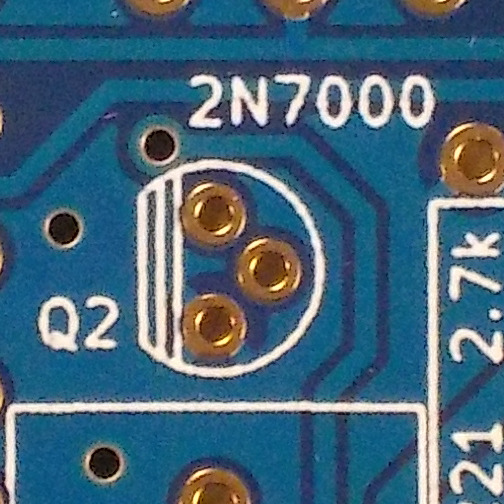
\includegraphics[width={1.50in}]{to92-bar.jpg}\quad
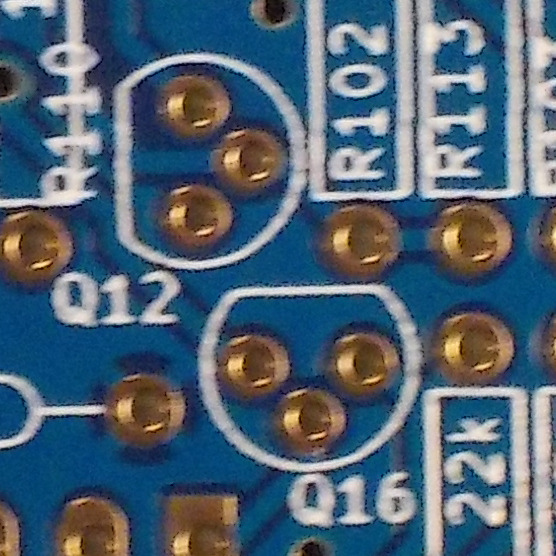
\includegraphics[width={1.50in}]{to92-nobar.jpg}

All TO-92 components in this project are polarized and must be installed in
the correct orientation to work; that orientation is shown by the silkscreen
symbols.  Install each component so that its flat side points in the same
direction as the flat side shown on the silkscreen.  The three legs of the
component must be carefully bent into the same triangular pattern (left and
right forward, middle backward) as the holes on the board, and then the
component pressed into place.  There should be a gap of about three
millimetres between the board and the component body; do not attempt to seat
the component flush on the board because of the risk of breaking off the
legs where they enter the body.

The solder pads for these components are smaller and closer together than
for any other through-hole components in the project, and the components
themselves tend to be relatively heat-sensitive.  Solder them carefully,
avoiding creating any solder bridges between adjacent pads.  Do not use
excessive time and heat trying to get the solder to flow through the board
and fillet on both sides, especially not on pads connected to the ground
plane; two-sided fillets may happen naturally, but it is enough for solder
to completely cover the pad on one side.  Excess heat on the pads in the
sine shaper, in particular, causing pads to lift off the boards, was a
significant problem in some of my prototype builds with rush-production
boards.  The boards supplied in kits ought to be higher quality and have
less risk of this issue, but it still requires caution.

\pagebreak

Install the thirteen 2N3904 transistors Q4--Q16.  These make up the core of
the sine shaper:  a grid of twelve transistors that correspond to different
voltage levels in the input, and one more transistor used as a current
source to provide the reference current that the others will switch to
different busses.

\nopagebreak
\noindent\includegraphics[width=\linewidth]{{2n3904}.jpg}

Install the two 2N7000 MOSFETs Q2 and Q3.  These are low-resistance switches
used in the triangle to sawtooth shapers.  As described above, they are
static-sensitive until successfully installed.

\nopagebreak
\noindent\includegraphics[width=\linewidth]{{2n7000}.jpg}

One TO-92 component should be left over after building Board~2:  the 78L09
regulator that will be installed later on Board~1.

\section{More capacitors}

Install the nine 100pF ceramic capacitors C10--C12, C24--C26, and C39--C40. 
These are compensation capacitors used to ensure stability on op amps that
have outputs exposed to the outside world.  They are unpolarized and may be
installed in either orientation.  Note that although this photo shows yellow
capacitors that were used in early assembled-module builds, most kits will
ship with blue capacitors.  The capacitors are likely to be marked ``101''
for the digits 10 followed by one more 0, that is 100, number of picofarads
(much like the resistor code).

\nopagebreak
\noindent\includegraphics[width=\linewidth]{{cap-100p}.jpg}

Install the two 1200pF film capacitors C5 and C19.  These are the timing
capacitors for the oscillator cores.  They are unpolarized and may be
installed in either direction.  The markings on film capacitors vary
depending on the manufacturer and model.

\pagebreak
These ones might be marked ``122''
(for 12 followed by two 0s number of picofarads),
``1n2'' (for 1.2nF), or even ``0.0012'' (value in $\mu$F).

\nopagebreak
\noindent\includegraphics[width=\linewidth]{{cap-1200p}.jpg}

Install the two 10$\mu$F electrolytic capacitors C29 and C30, which
filter the power supply for the module as a whole. 
These are polarized components and they may explode if installed backwards. 
Each one will be marked on its casing with a stripe and minus signs to
indicate the negative lead; the positive lead will probably also be longer. 
These clues should be matched with the markings on the PCB: plus and minus
symbols in the silkscreen and a square solder pad for the positive (long)
lead.  There should be one more 10$\mu$F electrolytic capacitor remaining,
for use on Board~1.

\nopagebreak
\noindent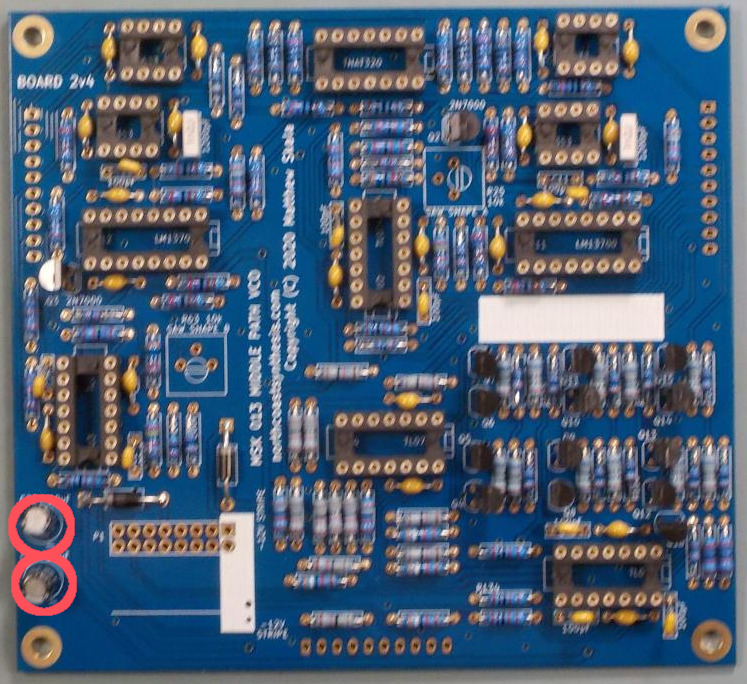
\includegraphics[width=\linewidth]{cap-10u2.jpg}

\section{Trimmer potentiometers}

Trimmers usually are not washable, so if you plan to clean your boards by
full immersion in water or other solvent, your last chance is now; future
cleaning will have to be done with a brush and some care to avoid letting
liquid seep into the trimmers.  Even now you should take some care with the
DIP sockets, because although they are in principle washable, solvent can
carry flux residue into the sockets and form a varnish-like layer if not
carefully rinsed away.

Trimmers are not exactly polarized, but the three legs of each trimmer serve
different functions and need to be connected to the right holes.  The
physical arrangement of the legs and corresponding holes should make it
impossible to install the trimmers wrong way round.

Install the two 10k$\Omega$ single-turn trimmers R25 and R63.  These trimmers
adjust the voltage offset between the first and second halves of the
sawtooth wave, so that you can null out the glitch where the halves join.

\nopagebreak
\noindent\includegraphics[width=\linewidth]{{trim-10k}.jpg}

\section{Eurorack power connector}

Install the 2$\times$8-pin Eurorack power connector P1.  This connector is
polarized, and although the pad footprint is symmetrical, installing the
connector in anything but the correct orientation would cause it to
interfere with the Schottky diodes, so there is little risk of getting it
wrong.  As with the DIP sockets, you should be careful to get it installed
snugly against the board, not tilted at an angle.  Use tape or putty to hold
it in place, solder one pin, then check that it is straight before you
solder the other pins.

Beware of solder bridges among the pins of the 16-pin power connector.  Many
of the pins are deliberately connected together anyway, and bridges among
those pins are harmless enough, but unless you are sure you know which ones
the connected-together pins are, it is advisable to remove all solder
bridges.  I recommend using a wider tip on the soldering iron because the
connector pins are heavy and require more heat than most other components,
but it remains important not to use excessive heat and damage the board.

\nopagebreak
\noindent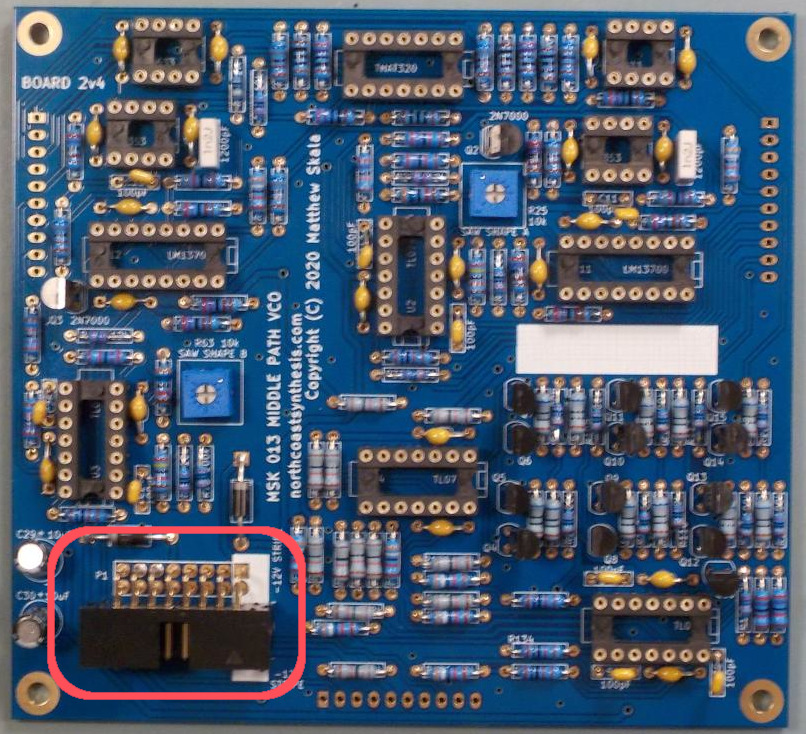
\includegraphics[width=\linewidth]{power.jpg}

A little more assembly is required for Board~2, namely installing the pin
headers for connecting to Board~1, and inserting the DIP ICs in their
sockets, but it is more convenient to do those steps later as part of the
Board~1 and final assembly.

In between completed boards is a good time to take a break.
